
\section{Introduction: Sound in the Language of Linear Algebra}

\par \indentt The core essence of musicianship has been hotly debated for millennia. Is technique the essential ingredient? Is emotion? Is it simply raw talent?

\par \bigskip No. The core essence of musicianship is looking cool, and there are few better ways to look cool than turning knobs on your instrument. Confident knob-turning signals competence to one's audience. A musician may practice scales and arpeggios until their eyes cross, but knob-turns truly make or break their performance.

\par \bigskip What are musicians really doing to their sound when they turn knobs? That question is the motivation for this paper. It turns out that they are applying linear transformations called \textbf{filters} to periodic functions, the properties of which are very useful for the music-making process. I will guide the reader from intuitive concepts of sound to a concrete mathematical understanding of the use of filters in music.

\subsection{Mechanics of Sound}

\par \indentt Sound waves are vibrations which travel through the air as molecules bump into each other, eventually hitting our ear drums and causing them to vibrate. We can represent this process mathematically with a \textbf{signal}, a function that describes some phenomenon. A simple vibration from a single source is called a \textbf{pure tone}, and its signal is a periodic function of pressure applied to the eardrum against time. Figure \ref{fig:pure_tone} demonstrates how the graph of this function takes a sinusoidal shape.\cite{Pierce} Thus, the signal for a pure tone is $f(t) = a\sin(\frac{2\pi t}{T})$, or perhaps $f(t) = a\cos(\frac{2\pi t}{T})$. \\

\begin{figure}[h]
    \centering
    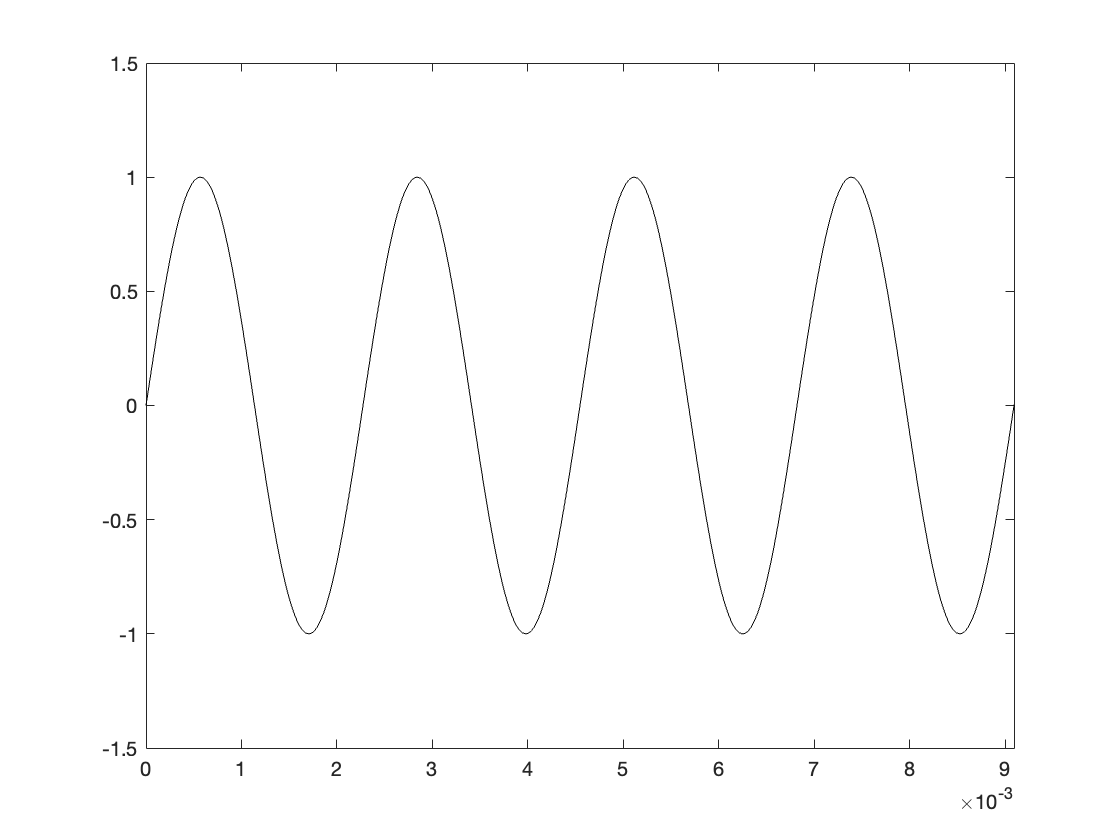
\includegraphics[scale=.15]{pure_tone_A4.png}
    \caption{A \href{https://drive.google.com/file/d/1Kkbf2dlfvdJgidkY80bJVJJ9kDVgS8sk/view?usp=sharing}{\color{blue} $[\blacktriangleright]$~pure tone} with amplitude $a = 1$ and period $T = \frac{1}{440}$ seconds}
    \label{fig:pure_tone}
\end{figure}

\par Since the function $f(t) = \sin(t)$ has a period of $2\pi$, it is useful to use pure tones whose frequencies are multiples of $2\pi$, which ``standardizes" the period. The pure tone $\sin(2\pi(1)t)$ has period $T = 1$, while $\sin(2\pi(\frac{1}{2})t)$ has period $T = 2$, and so on.

\newpage

\par \noindent A pure tone can be described when two\footnote{Strictly speaking, a third variable is necessary to describe a pure tone completely: its \textbf{phase} is the location of its peak amplitude. For a few examples, the phase of $\cos(2\pi t)$ is 0, the phase of $\sin(2\pi t)$ is 0.25, and the phase of $\sin(2\pi(t-0.6))$ is $.25-(-0.6) = 0.85$. \par Since a pure tone is a periodic function, its overall form remains the same as it is repeated over and over. Thus, a change of phase does not affect our auditory experience of a pure tone, and it is not very relevant for the following.} variables are known:\cite{Pierce}

\begin{itemize}
    \item The \textbf{amplitude} $a$ of the pure tone is the vertical distance between 0 and the peak of the sine wave, or the maximum pressure. Amplitude determines how loud the pure tone is, with higher values corresponding to louder sounds.
    \item The \textbf{period} $T$ of the pure tone is how long the sine function takes to complete one cycle. Alternatively, we can use the \textbf{frequency} $\nu = \frac{1}{T}$ to describe this aspect of the pure tone, in which case the equation is $f(t) = a\sin(2\pi\nu t)$. Frequency determines the \textbf{pitch} we hear from the pure tone. For example, the pitch of a pure tone with frequency $\nu = 440$ Hertz (Hz) is known as A4.
\end{itemize}

\par All around us, vibrations generate pure tones of different amplitudes and frequencies.\footnote{After the mechanical force producing them is done happening, sounds decay in amplitude over time. We get ``sustained" periodic tones from sustained vibrations. Wind instruments and traditional organs sustain tones by blowing air at a consistent rate through a pipe, while bowed instruments vibrate strings for the same effect. In contrast, ``plucked" tones are produced by short vibrations from a guitar or piano or some such, decaying quickly thereafter. Though plucked tones can be filtered, we will focus on the easier task of filtering sustained tones.} When they reach our ears simultaneously, the vibrations compound each other, and the signal for the pressure on our eardrum is the sum of the pure tone signals.\cite{Pierce} If enough pure tones are happening, their sum can sound like any continuous periodic function imaginable. We can even use pure tones to construct sounds that represent non-continuous functions, such as the square and sawtooth waves shown in Figure \ref{fig:square_sawtooth}. How is this possible without breaking the laws of physics? Stay tuned.

\begin{figure}[h]
    \centering
    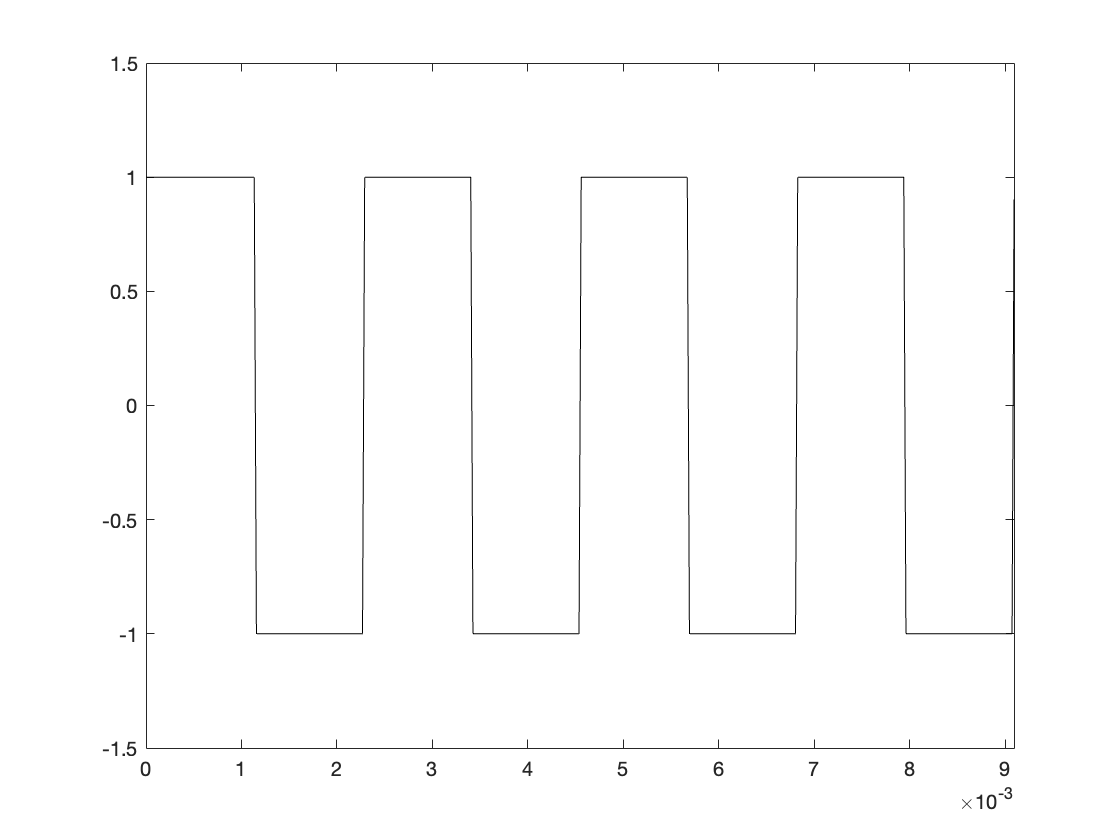
\includegraphics[scale=.15]{square_A4.png}
    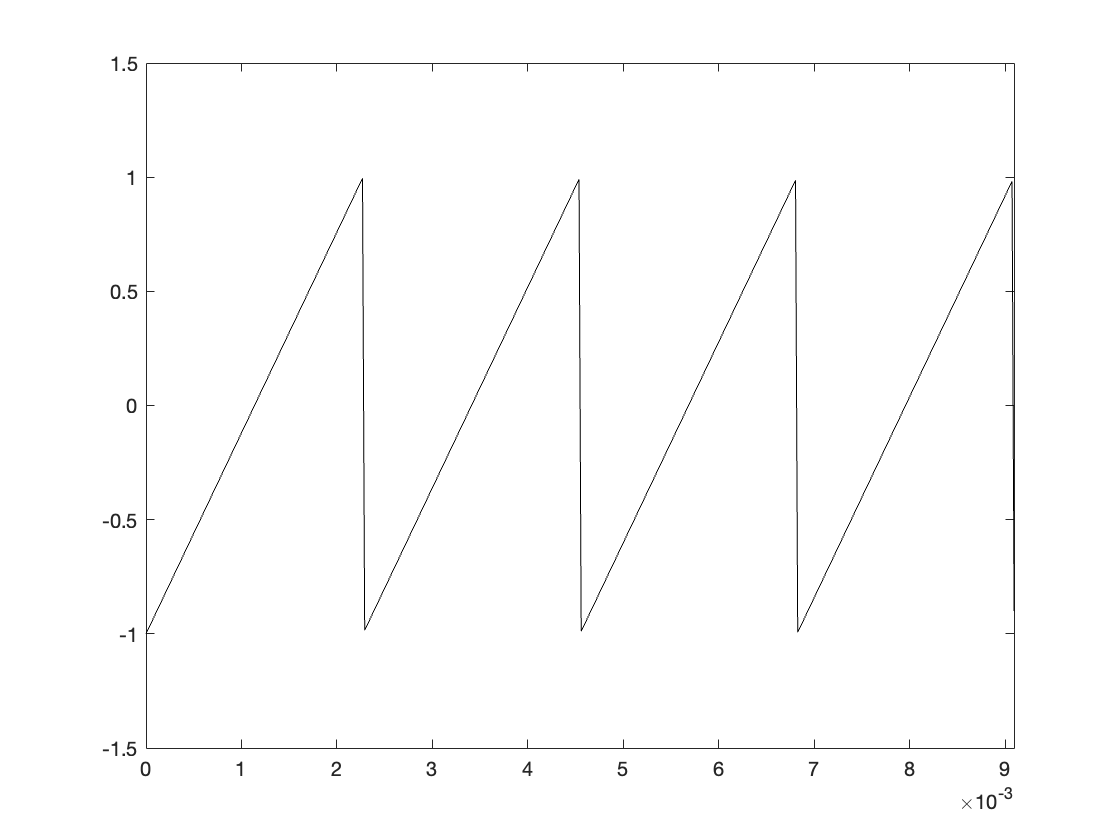
\includegraphics[scale=.15]{sawtooth_A4.png}
    \caption{\href{https://drive.google.com/file/d/1258wPS87kcBCvN_tSSiJX62L3gxTmrCi/view?usp=sharing}{\color{blue} $[\blacktriangleright]$~Square} and \href{https://drive.google.com/file/d/12ifgK4XE0z8f6byHCA4ULdHENxMqbqqZ/view?usp=sharing}{\color{blue} $[\blacktriangleright]$~sawtooth} waves with amplitude $a = 1$ and period $T = \frac{1}{440}$}
    \label{fig:square_sawtooth}
\end{figure}

\subsection{Sound as a Linear System}

\par \indentt A set of pure tones with specified frequencies can be thought of as a vector that represents a sound. It follows that the collection of all sounds has the properties of a vector space. To verify this, we must rigorously define the following operations on vectors of pure tones:

\begin{itemize}
    \item \textbf{Addition:} When two pure tones $\vecv$ and $\vecw$ hit the eardrum simultaneously, their forces combine to apply the pressure-over-time function $f(t) = \vecv+\vecw$. In other words, we do not experience the two pure tones separately, but as one wave with varying amplitude across the period.
    \item \textbf{Scalar multiplication:} Scaling a pure tone $c\cdot\vecv$ makes it $c$ times louder.
    \item \textbf{Negation:} Scaling a pure tone $\vecv$ by $-1$ reflects the sine or cosine function across the time axis. This negated pure tone has the same frequency and amplitude, but its peak is displaced by $\frac{T}{2}$, so our auditory experience is virtually unchanged.
\end{itemize}

\par Finally, let the vector $\vecz$ correspond to a silent wave with amplitude $0$. Under these definitions, the set of pure tones qualifies as a vector space. Table \ref{tab:axioms} provides intuitive explanations of the associative, commutative, and distributive properties of this pure tone vector space. The mathematical truth of each statement can be verified easily by replacing each vector in the left column with $\sin(\frac{2\pi t}{T})$ or $\cos(\frac{2\pi t}{T})$ for some $T\in\real$.

\begin{table}[!h]
    \centering
    \begin{tabular}{|l|l|l|}
        \hline
        Axiom & Intuitive Explanation\\
        \hline
        $\vecv+\vecw = \vecw+\vecv$ & Sustaining the pure tone $\vecv$ and then playing $\vecw$ produces \\& the same sound as playing $\vecw$ and then $\vecv$. \\
        \hline
        $(\vecu+\vecv)+\vecw =$  & Playing the sound that results from combining $\vecu$ and $\vecv$, \\ $\vecu+(\vecv+\vecw)$ & then adding $\vecw$ is the same as playing $\vecu$, then the \\& combination of $\vecv$ and $\vecw$.\\
        \hline
        $\vecv+\vecz = \vecv$ & Playing $\vecv$ and then silence is the same as just playing $\vecv$.\\
        \hline
        $\vecv+(-\vecv) = \vecz$ & If one pure tone is pushing the eardrum one way while \\& the other pushes it the opposite way the same amount, \\& they will entirely cancel each other out.\\
        \hline
        $1\vecv = \vecv$ & Amplifying a pure tone by a factor of 1 does not change \\& its loudness.\\
        \hline
        $c(d\vecv) = (cd)\vecv$ & Amplifying $\vecv$ by $d$, then by $c$ is the same as amplifying \\& $\vecv$ by $cd$.\\
        \hline
        $c(\vecv+\vecw) = c\vecv+c\vecw$ & Amplifying pure tones after combining them is no different \\& than amplifying them individually, then combining them.\\
        \hline
        $(c+d)\vecv = c\vecv+d\vecv$ & Clearly, $\vecv$ has the same frequency as itself, so adding it to \\& itself  simply increases the pressure applied to the ear.\\
        \hline
    \end{tabular}
    \caption{Axioms of the sound wave vector space}
    \label{tab:axioms}
\end{table}

\newpage

\par We can think of the sound that results from hearing multiple pure tones simultaneously as a \textit{linear combination of pure tones}. For example, if we hear $2\sin(\frac{2\pi t}{90})$, $-\frac{5}{3}\cos(\frac{2\pi t}{120})$, and $\frac{4}{7}\cos(\frac{2\pi t}{165})$ all at once, the pressure on our ear over time is given by $f(t) = 2\sin(\frac{2\pi t}{90}) - \frac{5}{3}\cos(\frac{2\pi t}{120}) + \frac{4}{7}\cos(\frac{2\pi t}{165})$.\footnote{The period of this function is however long it takes for all the pure tones to return to their starting point simultaneously; that is, 1 over the greatest common divisor of their frequencies. In this case, the three frequencies are 90, 120, and 165, so the period is $\frac{1}{15}$.} Readers who have worked with audio processing software will likely recognize the look of the third plot in Figure \ref{fig:cluster_sum}: amplitude-over-time graphs are common visual displays for audio clips.

\begin{figure}[h]
    \centering
    \begin{tabular}{ccc}
        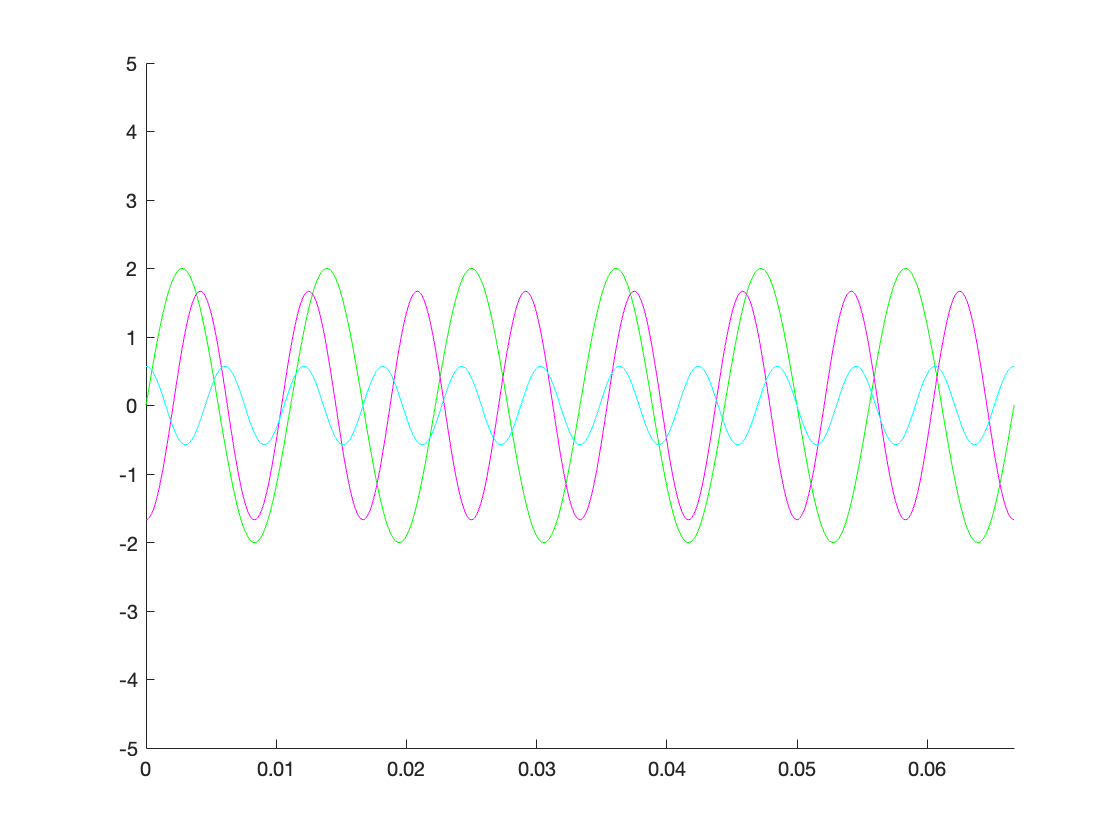
\includegraphics[scale=.125]{pure_tone_cluster.png} & 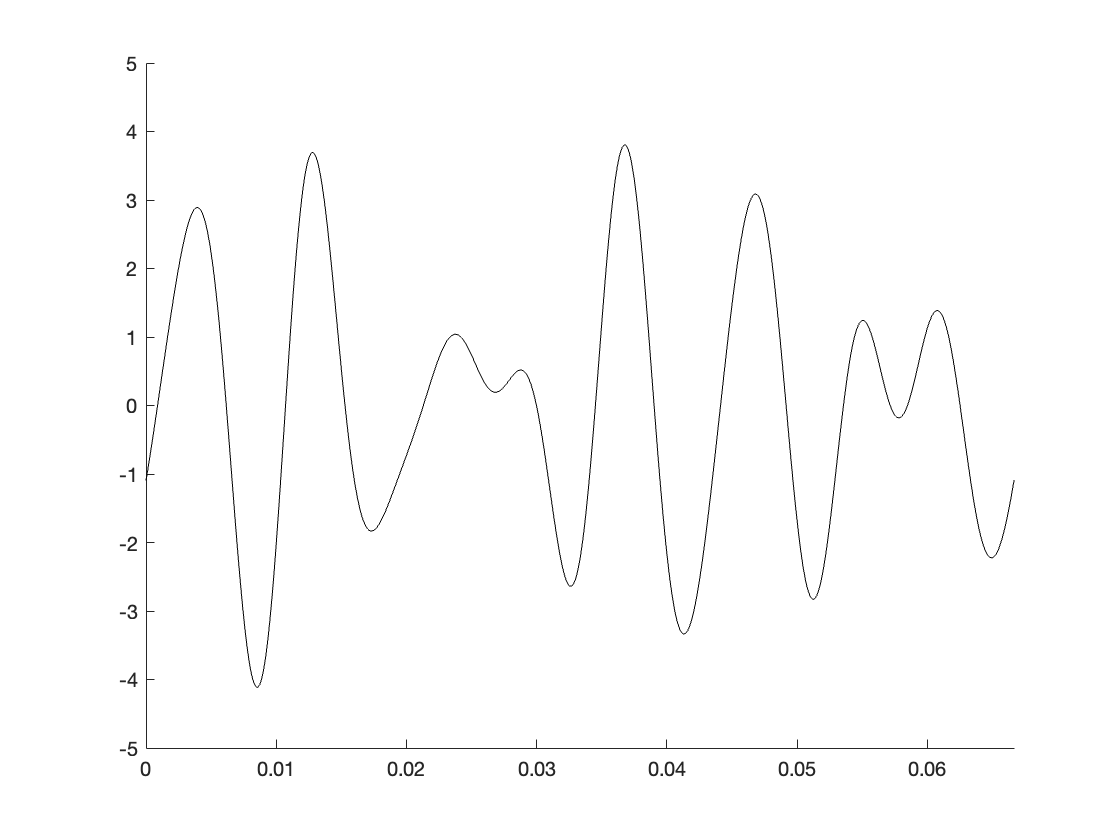
\includegraphics[scale=.125]{pure_tone_sum.png} & 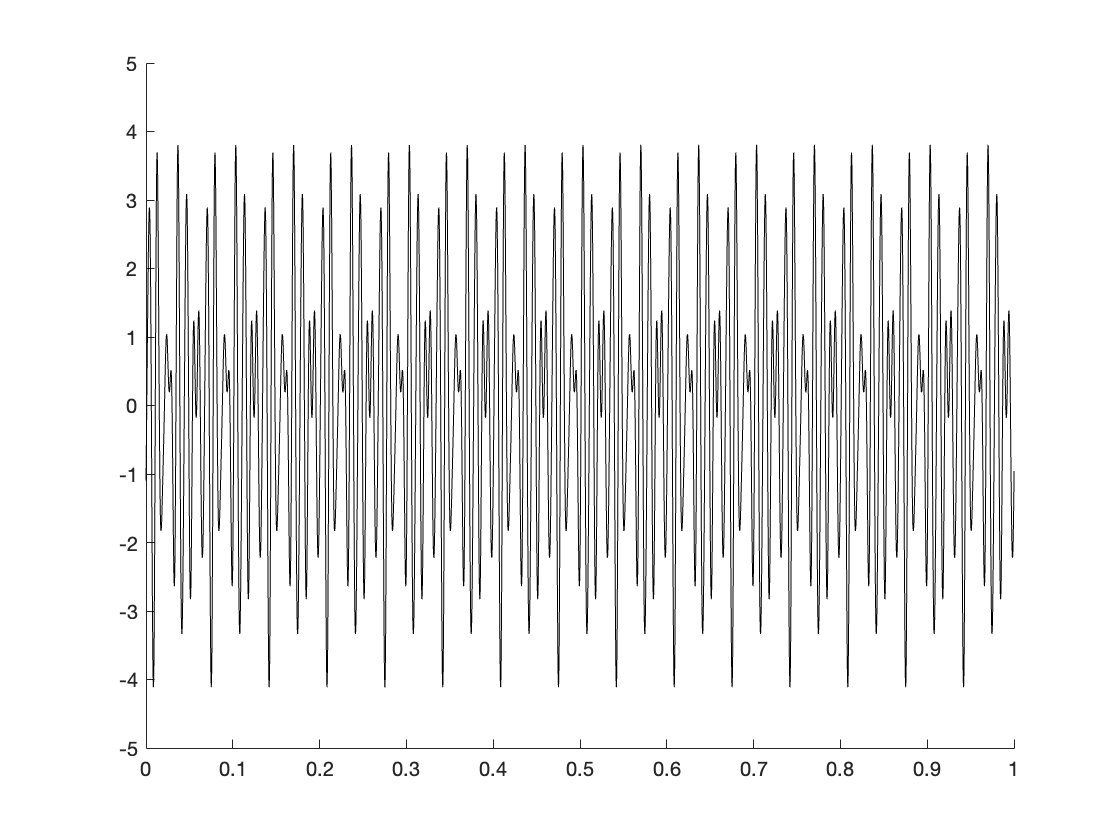
\includegraphics[scale=.125]{pure_tone_dense.png}\\
        Pure tones over $\frac{1}{15}$ seconds & $f(t)$ over $\frac{1}{15}$ seconds & $f(t)$ over 1 second\\
    \end{tabular}
    \caption{\href{https://drive.google.com/file/d/14drILSPmpc9H5VRfpYbGys3hszOjLL5u/view?usp=sharing}{\color{blue} $[\blacktriangleright]$~Three pure tones} and their \href{https://drive.google.com/file/d/1Qn-Je4ouRklJgiG2mEWmEwjWkEo9rs8y/view?usp=sharing}{\color{blue} $[\blacktriangleright]$~linear combination}}
    \label{fig:cluster_sum}
\end{figure}

\subsection{Musical Sounds}

\par \indentt Listen to the audio clips linked in Figure \ref{fig:cluster_sum}. You may notice that the three pure tones sound pleasant, while their linear combination sounds like garbage. Unfortunately, not every linear combination of pure tones produces a musical note. What property distinguishes a musical note from random noise?

\par \bigskip The answer lies in the ratios of pure tone frequencies. A musical note is a linear combination of pure tones whose frequencies are each equal to the lowest frequency, called the \textbf{fundamental frequency}, multiplied by an integer.\cite{Pierce} When such a family of frequencies is played simultaneously, our ears hear the pitch of the fundamental frequency. When $x$ unique frequency families are played together, we hear $x$ distinct notes. When the frequencies don't have nice ratios, we hear only muddled noise.

\par \bigskip Notes composed of fewer pure tones sound more pleasant and simple. This is a desirable quality for placid, soothing music, but musicians aim to evoke a much wider variety of emotions with their music. The relative amplitudes of the frequencies change the note's emotional characteristics, which together are called the \textbf{quality of sound}. We will refer to notes with the same pitch but different sound qualities as different \textbf{tones}. As we shall see, filters alter a note's sound quality without changing the frequencies of its pure tones, i.e. they change tone without changing pitch, making them quite useful for musicians.